\documentclass[tikz,border=14pt]{standalone}
\usepackage{amsmath,amssymb}
\usetikzlibrary{arrows.meta}
\definecolor{ink}{HTML}{E4EDF8}
\definecolor{muted}{HTML}{596B80}
\definecolor{blue}{HTML}{9FC2FF}
\definecolor{teal}{HTML}{63D3BB}
\definecolor{gold}{HTML}{E7C274}
\definecolor{panel}{HTML}{111923}
\pagecolor{panel}
\color{ink}
\begin{document}
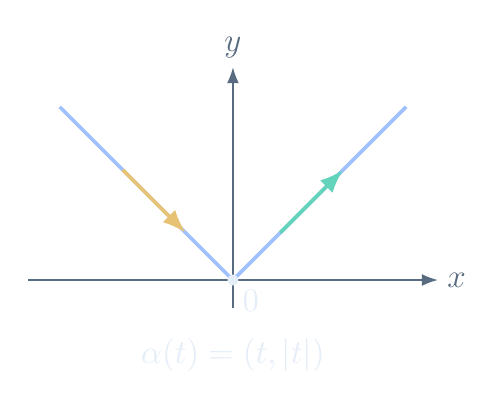
\begin{tikzpicture}[font=\large,text=ink,vec/.style={-{Latex[length=3mm]},line width=1.3pt},axis/.style={muted,-{Latex[length=2mm]},thin}]

\draw[axis] (-2.6,0)--(2.6,0) node[right] {$x$};\draw[axis] (0,-.35)--(0,2.7) node[above] {$y$};
\draw[blue,line width=1.3pt] (-2.2,2.2)--(0,0)--(2.2,2.2);
\draw[vec,gold] (-1.4,1.4)--(-.6,.6);\draw[vec,teal] (.6,.6)--(1.4,1.4);
\fill[ink] (0,0) circle(2pt) node[below right] {$0$};
\node at (0,-.95) {$\alpha(t)=(t,|t|)$};

\end{tikzpicture}
\end{document}
